\documentclass{article}
\author{}
\usepackage[utf8]{inputenc}
\usepackage{amsmath}
\usepackage{amssymb}
\usepackage{amsmath,amsthm,amssymb,scrextend}
\usepackage{fancyhdr}
\usepackage{graphicx}
\usepackage{hyperref}
\usepackage{float}
\usepackage{booktabs}
\usepackage[margin=2.5cm]{geometry}

% School name and logo
\newcommand{\schoolname}{Vietnam National University Ho Chi Minh City \\ Ho Chi Minh City University of Technology \\ Faculty of Computer Science and Engineering}
\newcommand{\schoollogo}{
\includegraphics[width=3cm]{img/hcmut.png}}

\begin{document}
\begin{titlepage}
    \centering
    \vspace*{2cm}
    \schoollogo\par
    \vspace{1cm}
    {\Large \schoolname\par}
    \vspace{3cm}
    {\huge\bfseries Internship I -\ Report \par}
    \vspace{1cm}
    {\Large\bfseries Supervisor: Assoc. Prof.\ Quan Thanh Tho \par}
    \vspace{1cm}
    {\large \bfseries Tang Quoc Thai -\ 2270376\par}
    \vfill
    {\large \today\par}
\end{titlepage}

\section{Motivation}
The project is motivated by the overarching objective of empowering Bahnaric language speakers, with a primary focus on enhancing communication within their ethnic community and fostering interaction with other ethnic groups. Recognizing the significance of precise phoneme segmentation in linguistic analysis, the project aims to establish a detailed phoneme-level mapping for the Bahnaric language. This mapping not only holds intrinsic linguistic value but also serves as a pivotal foundation for the development of advanced Text-to-Speech (TTS) and Automatic Speech Recognition (ASR) models tailored to the unique phonetic characteristics of the Bahnaric language. The overarching goal is to contribute meaningfully to the empowerment and connectivity of Bahnaric ethnic communities, leveraging targeted advancements in speech processing for the benefit of language preservation and inter-community communication.
\section{Theoretical Background}
\subsection{Phoneme Segmentation}
\begin{sloppypar}
Detecting phoneme boundaries or segmenting phonemes is a crucial initial step in various speech processing applications, including speaker diarization~\cite{moattar2012review}, speech science~\cite{adi2016automatic, adi2015vowel}, keyword spotting~\cite{keshet2009discriminative}, Automatic Speech Recognition~\cite{kubala1996transcribing, rybach2009audio}, and more. These segmentations are typically achieved through supervised or unsupervised methods. In the unsupervised approach, only the speech signal is used as input~\cite{michel2016blind, sorin2006relation}, while in the supervised approach, the speech signal is accompanied by target boundaries for guidance. In supervised scenarios, the set of pronounced or presumed phonemes is often provided as additional input, known as forced alignment. When no phonemes are supplied, the setup is termed text-independent phoneme segmentation~\cite{aversano2001new, chen2016text}. This study specifically focuses on the supervised text-independent phoneme segmentation problem.
\end{sloppypar}
\begin{figure}[H]
    \centering
    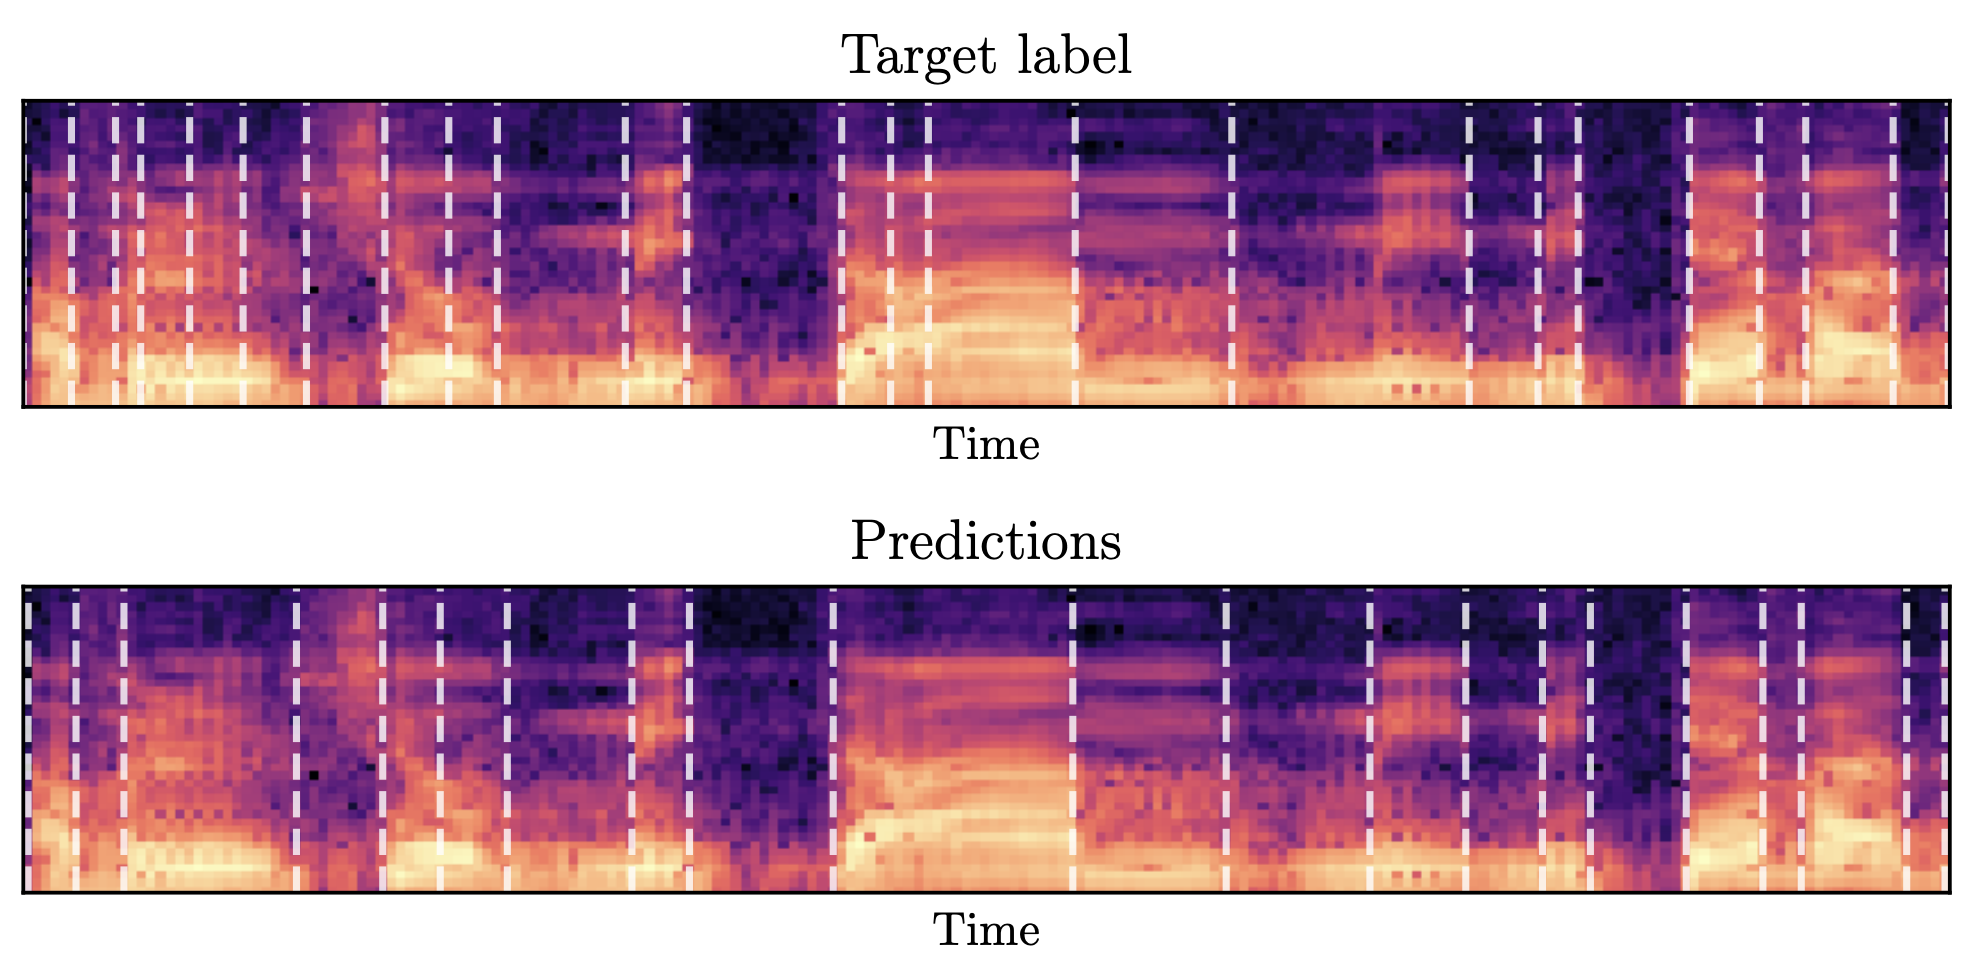
\includegraphics[width=0.8\textwidth]{img/phoneme_boundary_detection.png}
    \caption{Example of supervised phoneme boundary detection.}
\end{figure}
\subsection{Related Works}
\begin{sloppypar}
Researchers have delved into the challenge of detecting phoneme boundaries across different scenarios. In the unsupervised setting, also termed blind phoneme segmentation, the speech signal is presented without any additional phonemes or boundaries for guidance. Traditionally, signal processing techniques were utilized to identify spectral changes in the signal for phoneme boundary detection~\cite{dusan2006relation, estevan2007finding, hoang2015blind, almpanidis2008phonemic, rasanen2011blind}, as mentioned in the respective references. A recent proposal in~\cite{michel2016blind} suggests training a next-frame prediction model using an approximated Markov model or RNN to pinpoint potential phoneme transitions in regions of high error.\\[5mm]
In the supervised setting, the forced alignment approach is prevalent. Models employing this approach typically involve Hidden Markov Models or various structured prediction algorithms with handcrafted features~\cite{keshet2005phoneme, mcauliffe2017montreal}. However, a significant drawback of forced alignment methods is the necessity for phoneme annotations even during inference, limiting their applicability to monolingual settings due to potential mismatches in phoneme sets from foreign languages.\\[5mm]
Another supervised setting is text-independent phoneme boundary detection, where the model receives phoneme boundaries as supervision but lacks information about the uttered phonemes. In previous works following this setup, the problem is often treated as a binary classification task, associating one label with phoneme boundary annotations and another with the remaining signal. For instance, in~\cite{king2013accurate}, a kernel-based method consisting of six radial basis function support vector machines was employed, while~\cite{franke2016phoneme} suggested using an RNN followed by a peak detection algorithm for predicting phoneme boundaries. However, a drawback of such modeling is the neglect of the internal structure of the output, treating boundaries as conditionally independent.\\[5mm]
Additionally, noteworthy are related lines of work in the domain of learnable segmental features in ASR~\cite{lu2016segmental}, dependency parsing~\cite{kiperwasser2016simple}, and word segmentation~\cite{adi2017sequence}.
\end{sloppypar}
\section{Proposed Method}
\subsection{Data Preprocessing}
\begin{sloppypar}
Parselmouth, accessible at \href{https://parselmouth.readthedocs.io/en/stable/}{link}, is a Python-based library designed for the extraction of speech features. It leverages Praat, a free, open-source software for speech synthesis and analysis, as its feature extraction backend. Parselmouth offers a Python-friendly interface to Praat's scripting language. In this project, Parselmouth was utilized to read the TextGrid file and extract the labeled marks `op' and `ov'.
\end{sloppypar}
\begin{figure}[H]
    \centering
    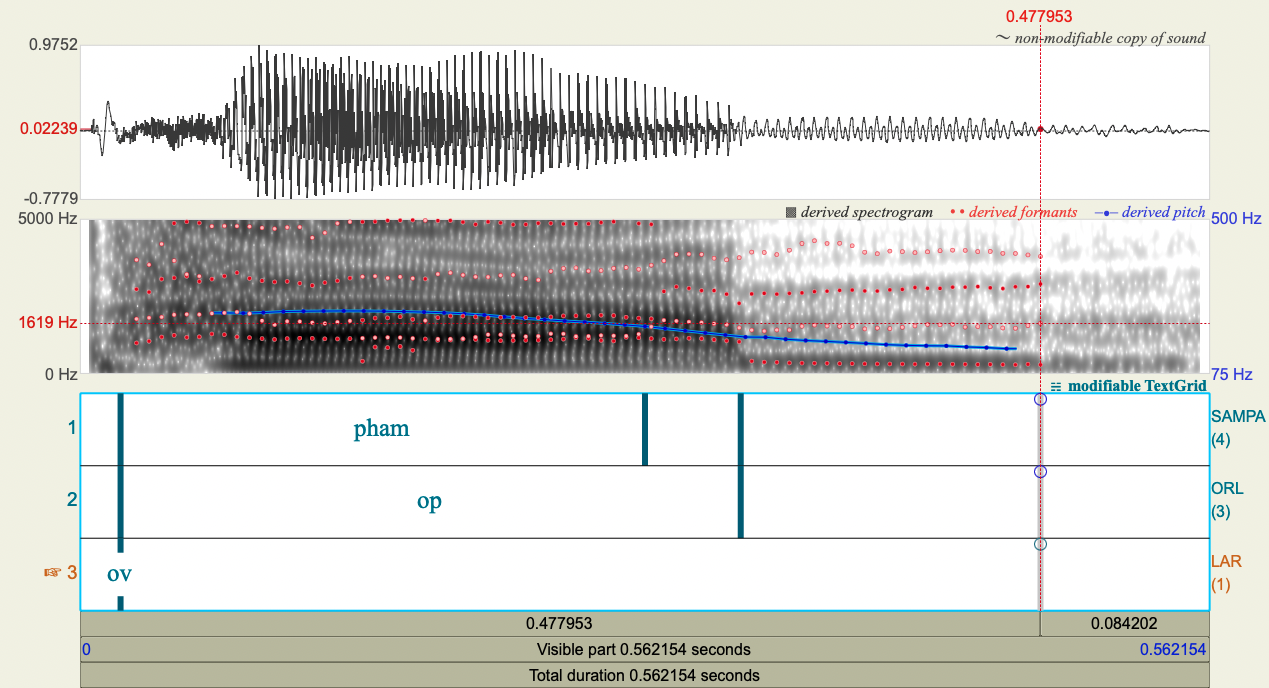
\includegraphics[width=0.8\textwidth]{img/phoneme_example.png}
    \caption{Example of labelled marks.}
\end{figure}
\subsection{Feature Extraction}
In the quest for proficient phoneme boundary detection, the intricate nature of deep learning meta-features, mainly when applied to ethnic languages, posed a challenge due to their complexity. Despite notable advancements in deep learning, a nuanced comprehension of these meta-features still needs to be discovered. To surmount this challenge, a judicious integration of theoretical knowledge with practical experience guided the selection of an acoustic feature-centric approach. The rationale behind this choice is that incorporating contextual understanding enhances the model's ability to discern phoneme boundaries in the specific linguistic context. The list of acoustic features used in this project is as follows:
\begin{itemize}
    \item Zero-crossing rate
    \item Spectrogram statistics
    \item Harmonic and perceptual features
    \item Chroma representations
    \item Tempo in BPM
    \item Spectral characteristics
    \item Bandwidth measures
    \item MFCCs
\end{itemize}
Additionally, the variability in time series data length arising from acoustic feature calculations necessitated a strategic response. To address this, a sophisticated technique involving diverse window sizes was employed. By calculating the average of the time series within each window, a uniform representation for each data point was achieved, fostering consistency in subsequent analyses. The resulting audio feature set comprises a comprehensive array, encompassing pivotal aspects such as zero-crossing rate, spectrogram statistics, harmonic and perceptual features, chroma representations, tempo in BPM, spectral characteristics, and bandwidth measures. This meticulous approach accommodates the idiosyncrasies of ethnic languages, ensuring a nuanced and effective representation of phoneme boundaries within the task's framework.
\begin{figure}[H]
    \centering
    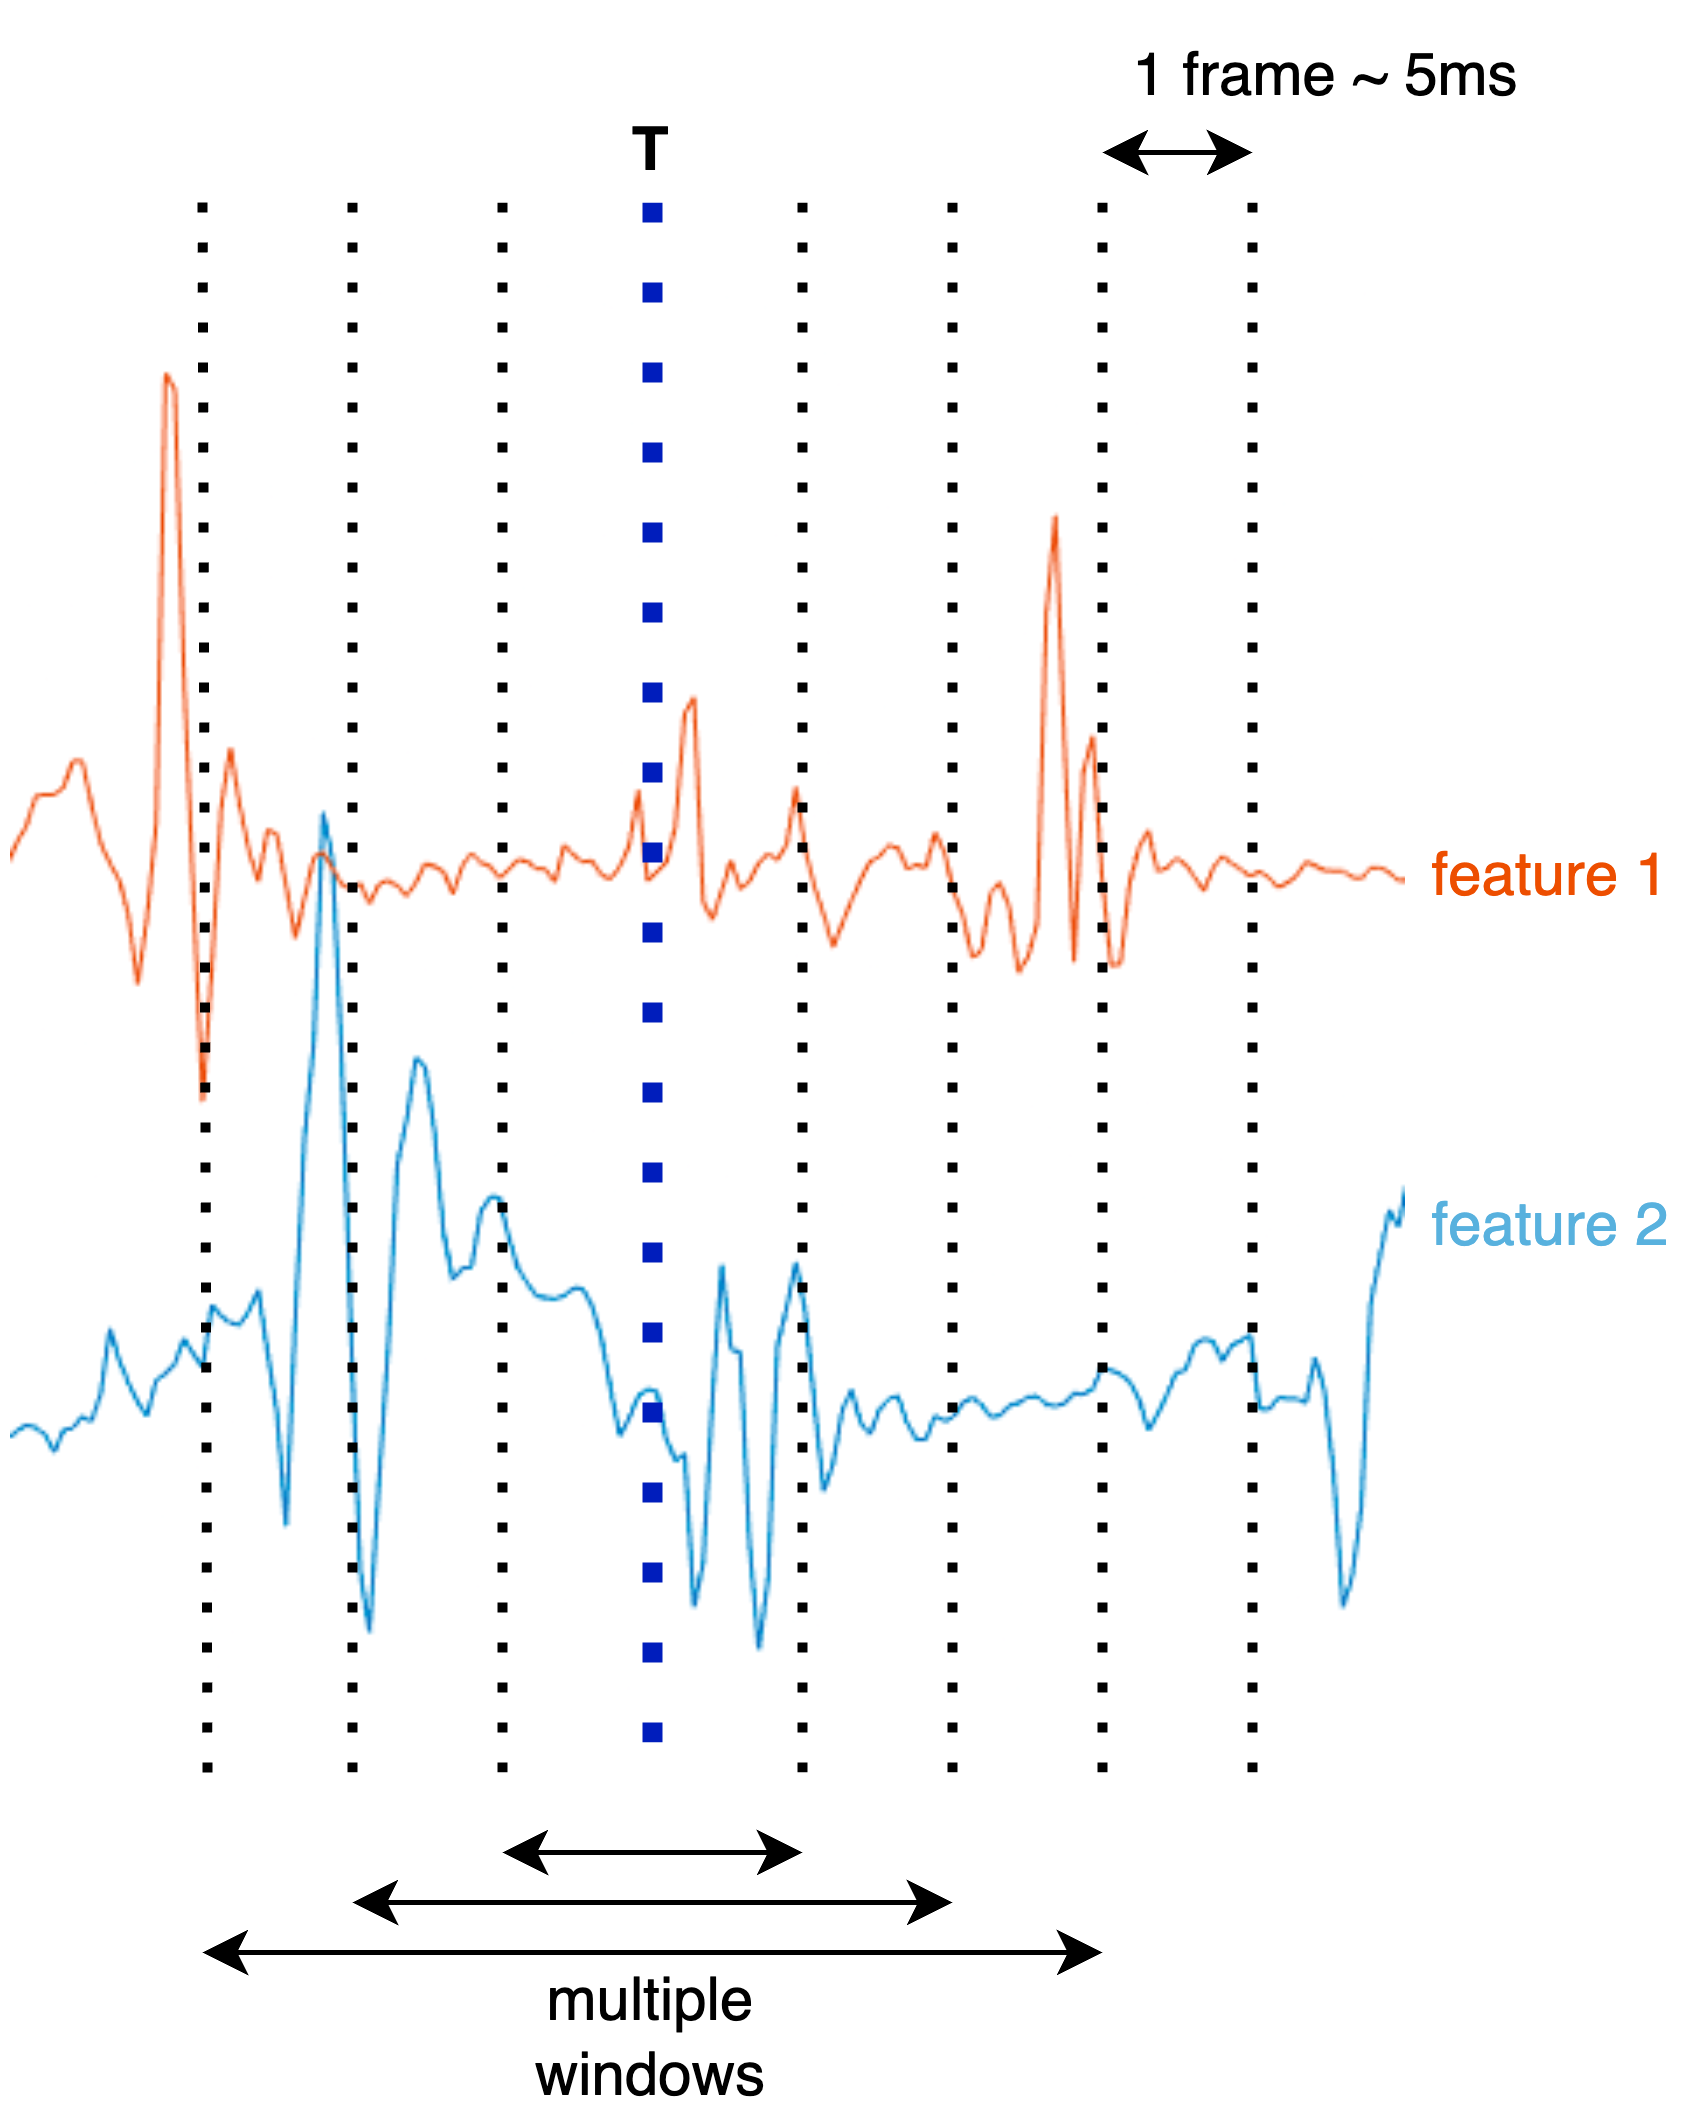
\includegraphics[width=0.6\textwidth]{img/features.png}
    \caption{Feature extraction method with multiple windows.}
\end{figure}
\section{Experiments}
Within a single audio file, the number of frames can reach several hundreds, whereas there exists only one `op' and one `ov' label. This results in a highly imbalanced dataset. To address this imbalance, a strategy is employed wherein the frames neighboring the true labels are also considered as potential labels. This approach serves to augment the label count, effectively mitigating the skewness in the dataset.
\begin{figure}[H]
    \centering
    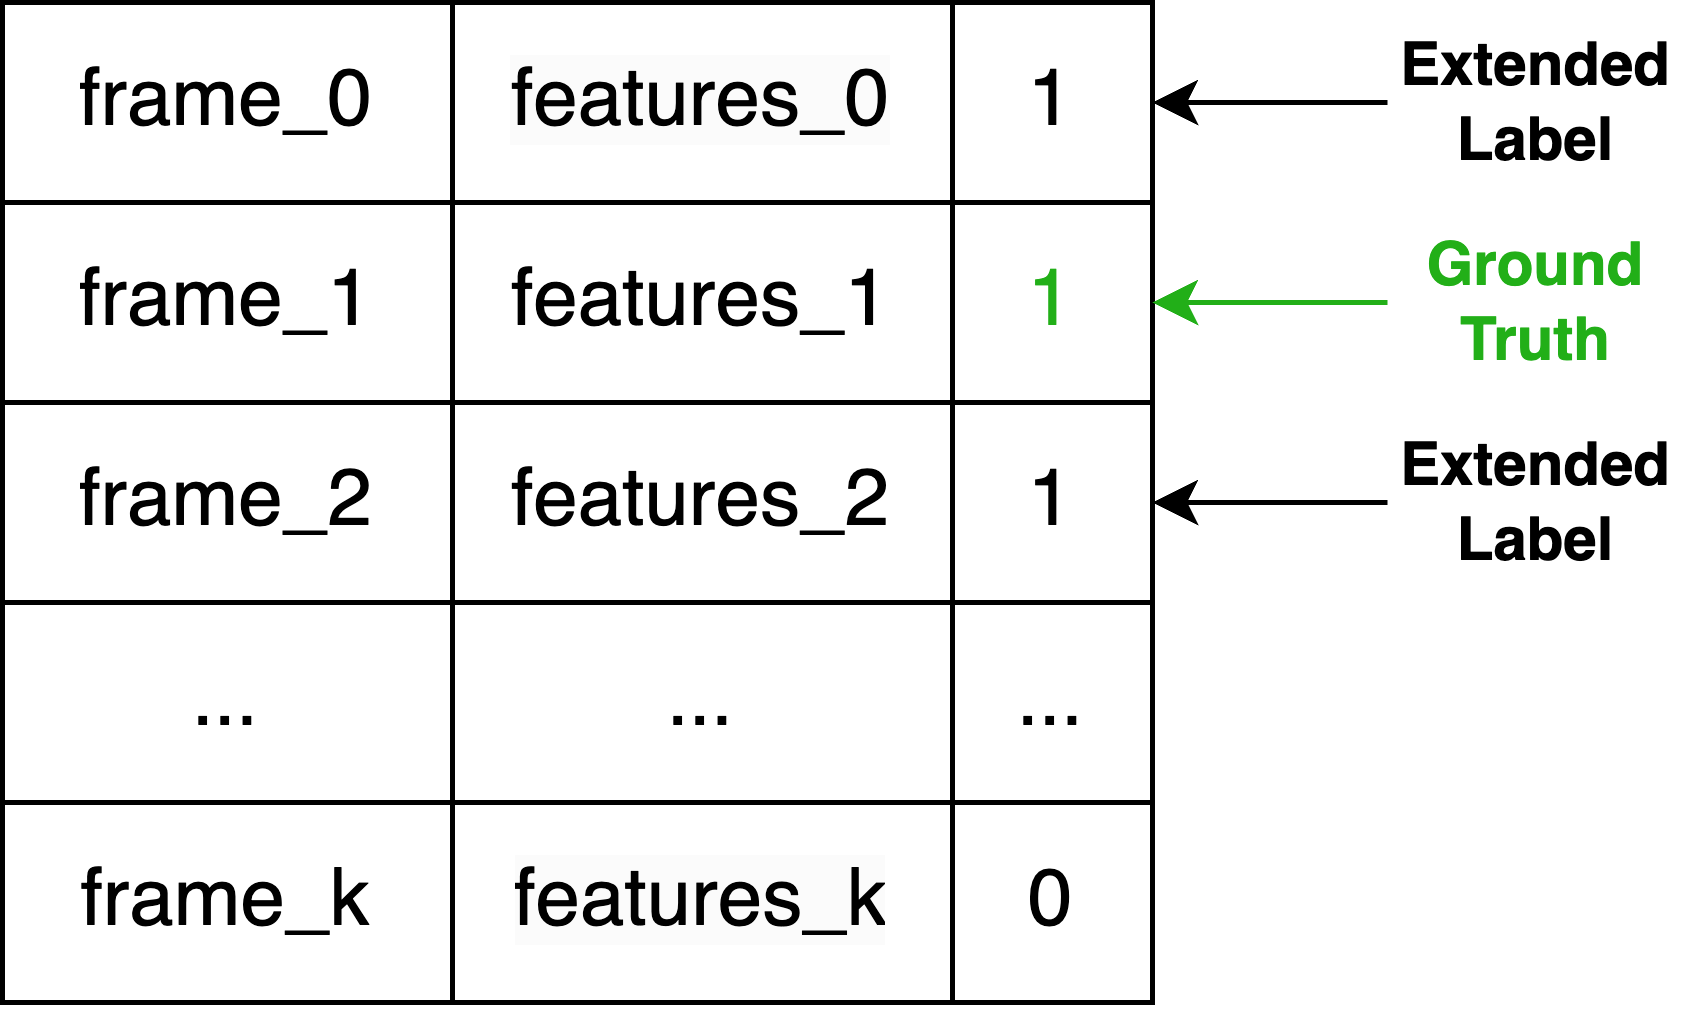
\includegraphics[width=0.6\textwidth]{img/training.png}
    \caption{Allow neighboring frames of the ground truth as extended labels.}
\end{figure}
The LightGBM model was trained on the dataset with default parameters, and the evaluation metrics are as follows:
\begin{table}[h]
    \centering
    \begin{tabular}{l c c c}
    \midrule
    & Precision & Recall & Accuracy \\
    op & 0.78 & 0.38 & 0.67 \\
    ov & 0.76 & 0.60 & 0.79 \\
    \midrule
    \end{tabular}
\end{table}
\section{Conclusion}

While acknowledging that the evaluation metrics of the trained model may not be flawless, the method employed in processing acoustic features for phoneme boundary detection in the Bahnaric language has been introduced. This contribution serves as a foundational step, providing a starting point for subsequent research endeavors.\\[5mm]
The source code of this project is available at \href{https://github.com/tqtensor/bahnaric-phoneme}{link}.
\bibliography{references}
\bibliographystyle{unsrt}

\end{document}
